% !TeX program = pdflatex
\pdfmapfile{+t1-times.map}
\pdfmapfile{+t1-formata.map}
\pdfmapfile{+t1-giovannistd.map}
\documentclass{ieeeaccess}
\usepackage{cite}
\usepackage{amsmath,amssymb,amsfonts}
\usepackage{graphicx}
\graphicspath{{../pic/}}
\usepackage{textcomp}
\usepackage{bm}
\usepackage{array}
\usepackage{placeins}
\usepackage{float}

\newcommand{\citep}[1]{\cite{#1}}

\def\BibTeX{{\rm B\kern-.05em{\sc i\kern-.025em b}\kern-.08em
    T\kern-.1667em\lower.7ex\hbox{E}\kern-.125emX}}

\begin{document}
\history{Date of publication xxxx 00, 0000, date of current version xxxx 00, 0000.}
\doi{10.1109/ACCESS.2026.DOI}

\title{Multi-Task Temporal-Perception-Enhanced LPV-MPC for Path Tracking of a Diagonal Dual-Steer AGV}
\author{\uppercase{Author Name}\authorrefmark{1}}
\address[1]{Affiliation placeholder.}
\corresp{Corresponding author: Author Name (e-mail: email@example.com).}

\begin{abstract}

This paper proposes a multi-task temporal-perception-enhanced linear parameter-varying model predictive control (LPV-MPC) framework for path tracking of a diagonal dual-steer automated guided vehicle (AGV) under sloped and turning-transition operating conditions, with abnormal resistance included as an auxiliary operating-condition perception target. In conventional LPV-MPC, inaccurate scheduling variables, especially slope-related information, may cause model mismatch and degrade closed-loop tracking performance. To address this issue, a lightweight ModernTCN-based temporal perception module is developed to estimate the operating condition, steering direction, and slope-related scheduling variable from a short history of proprioceptive measurements. The estimated information is incorporated into the online scheduling process of the LPV-MPC controller while retaining the constraint-handling capability and interpretability of the model-based controller. The proposed method is evaluated on a MATLAB/Simulink closed-loop simulation platform against zero-slope LPV-MPC, IMU-based LPV-MPC, true-slope oracle LPV-MPC, GRU, and conventional TCN baselines. The experiments include closed-loop baseline comparison, multi-route benchmarking, robustness tests under measurement noise and plant parameter perturbations, and a causal ModernTCN ablation. The results show that ModernTCN provides the most robust overall closed-loop performance among the learning-based methods, substantially improves tracking quality over non-AI scheduling baselines, and maintains its advantage across multiple routes and disturbance levels. These findings suggest that multi-task temporal perception is an effective scheduling enhancement for LPV-MPC, while also highlighting the necessity of closed-loop validation beyond offline perception metrics.

\end{abstract}

\begin{keywords}

Automated guided vehicle, closed-loop validation, diagonal dual-steer vehicle, linear parameter-varying model predictive control, ModernTCN, multi-task learning, path tracking, slope estimation, temporal perception.

\end{keywords}

\titlepgskip=-15pt
\maketitle

\section{Introduction}



\subsection{Background and Motivation}



\PARstart{A}{utomated} guided vehicles (AGVs) are widely used in factory logistics, warehouse transportation, and flexible manufacturing systems. In these applications, an AGV is required to track prescribed paths accurately while satisfying actuator constraints and maintaining smooth motion under varying operating conditions. Compared with conventional road vehicles, industrial AGVs often operate in confined spaces with frequent turning transitions, uneven ground, slope changes, load variations, and abnormal resistance. These factors may significantly affect the longitudinal, lateral, and yaw dynamics of the vehicle, especially when the vehicle adopts a multi-actuated steering and driving configuration.



This paper focuses on a diagonal dual-steer AGV, where the left-front and right-rear wheels are active drive-steer wheels, while the other two wheels serve as passive support wheels. This configuration provides good maneuverability for factory logistics routes, but it also introduces coupling among longitudinal motion, yaw motion, steering dynamics, and load transfer. Therefore, the path-tracking controller should not only reduce lateral and heading errors, but also maintain reasonable control smoothness and constraint satisfaction under sloped and transitional operating conditions.



Model predictive control (MPC) is a suitable control framework for constrained path tracking because it can explicitly consider future reference information, multi-variable dynamics, actuator limits, and input-rate constraints \citep{}. For nonlinear vehicle systems, linear parameter-varying MPC (LPV-MPC) provides a practical compromise between nonlinear model fidelity and online computational tractability \citep{}. By updating the prediction model according to measurable or estimable scheduling variables, LPV-MPC can adapt the local prediction model to different operating conditions without solving a full nonlinear optimization problem online.



\subsection{Scheduling Mismatch in LPV-MPC}



Although LPV-MPC is attractive for real-time vehicle path tracking, its closed-loop performance depends strongly on the accuracy of the scheduling variables. In the considered AGV system, the scheduling variables are not merely auxiliary signals. They directly influence the prediction model used by the MPC controller. In particular, the road slope affects the longitudinal resistance, load transfer, and the local dynamic model used in the LPV prediction. If the scheduled slope differs from the actual slope, the controller may predict an inconsistent vehicle response and generate unsuitable control actions.



This scheduling mismatch problem becomes more evident in factory routes that include slope changes, turning transitions, and possible abnormal resistance. A nominal zero-slope scheduler may be acceptable for flat-road operation, but it can become insufficient when the AGV enters a sloped segment. A simplified sensor-based slope estimate may also be biased by vehicle acceleration, transient pitch motion, sensor noise, or turning-induced coupling. Therefore, reliable scheduling information is important for improving the closed-loop quality of LPV-MPC.



The central problem considered in this paper is thus not how to replace LPV-MPC with a neural network controller, but how to enhance the scheduling process of LPV-MPC using temporal perception. The learning component is introduced as an auxiliary perception layer that estimates scheduling-related intermediate variables from historical proprioceptive measurements. The final control command is still generated by the constrained LPV-MPC controller.



\subsection{Temporal Perception as Scheduling Assistance}



Recent learning-enhanced MPC studies have shown that data-driven models can be combined with predictive control in several ways, such as learning vehicle dynamics, learning model residuals, estimating uncertainty, adapting cost and constraint parameters, or accelerating optimization \citep{}. In contrast to these approaches, this work learns interpretable scheduling-related perception variables for LPV-MPC. The learning module does not directly output the driving force command or yaw-rate command. Instead, it estimates the main operating condition, steering direction, and slope-related scheduling variable.



The proposed temporal perception module uses a short history of vehicle measurements rather than a single instantaneous signal. This design is motivated by the fact that slope transitions, stall-like abnormal resistance, and turning maneuvers are temporal phenomena. A window of recent acceleration, yaw rate, steering state, wheel speed, motor-current-related quantities, and derived diagnostic features can provide richer information than an instantaneous measurement. Based on this observation, a lightweight multi-task ModernTCN-based estimator is adapted for scheduling perception. The estimator jointly predicts the operating condition, steering direction, and slope-related scheduling quantity. The slope-related estimate is conditioned and incorporated into the LPV-MPC scheduler, while the classification outputs provide auxiliary operating-condition information for the multi-task representation. The overall structure of the proposed method is shown in Fig.~\ref{fig:overall_framework}.

% ===== Fig. 1 =====
\begin{figure*}[!t]
\centering
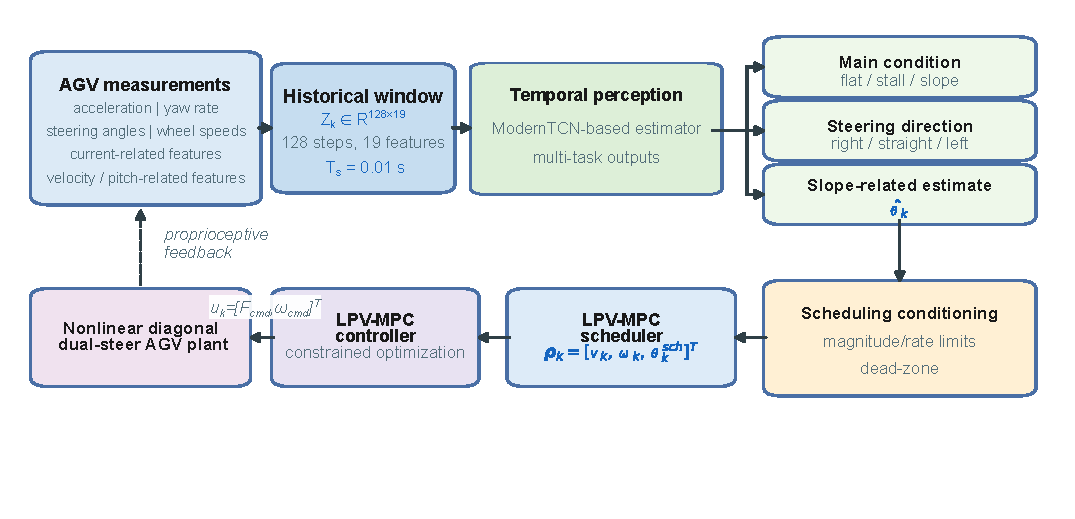
\includegraphics[width=\textwidth]{fig01_overall_framework.pdf}
\caption{Overall framework of the proposed temporal-perception-enhanced LPV-MPC. The ModernTCN-based estimator provides multi-task scheduling-related perception outputs from a historical proprioceptive window. The slope-related estimate is conditioned and incorporated into the LPV-MPC scheduling vector, while the final control commands are generated by the constrained LPV-MPC controller.}
\label{fig:overall_framework}
\end{figure*}
\FloatBarrier

\subsection{Contributions}



The main contributions of this paper are summarized as follows.


\begin{itemize}

\item A multi-task temporal-perception-enhanced LPV-MPC framework is proposed for diagonal dual-steer AGV path tracking under sloped and turning-transition operating conditions, with abnormal resistance included as an auxiliary operating-condition perception task. The learning module estimates interpretable scheduling-related variables rather than replacing the vehicle model, the MPC optimizer, or the control law.


\item A lightweight ModernTCN-based multi-task estimator is adapted for LPV-MPC scheduling perception. From historical proprioceptive measurements, the estimator jointly predicts the main operating condition, the steering direction, and the slope-related scheduling variable required by the LPV-MPC update.


\item A closed-loop simulation benchmark is established to evaluate the influence of scheduling perception on path tracking. The proposed method is compared with zero-slope LPV-MPC, IMU-based LPV-MPC, true-slope oracle LPV-MPC, GRU, and conventional TCN under the same nonlinear AGV plant and LPV-MPC controller.


\item A causal ModernTCN ablation is used to analyze the mismatch between offline perception metrics and closed-loop control quality. The result highlights that window-level classification and regression metrics are not sufficient for evaluating learning-enhanced MPC systems, and closed-loop validation is necessary.

\end{itemize}



\subsection{Paper Organization}



The remainder of this paper is organized as follows. Section~\ref{sec:related_work} reviews related work on MPC and LPV-MPC for vehicle path tracking, learning-enhanced MPC, AGV path tracking, and temporal neural networks. Section~\ref{sec:model_lpv_mpc} introduces the diagonal dual-steer AGV model and LPV-MPC formulation. Section~\ref{sec:temporal_perception} presents the multi-task temporal scheduling perception method. Section~\ref{sec:experiment_design} describes the simulation-based closed-loop experimental design. Section~\ref{sec:results_discussion} reports and discusses the closed-loop results, robustness tests, ablation study, and limitations. Section~\ref{sec:conclusion} concludes the paper.


\section{Related Work}

\label{sec:related_work}



\subsection{MPC and LPV-MPC for Vehicle Path Tracking}



MPC has been widely studied for vehicle and mobile robot path tracking because it can explicitly handle multi-variable dynamics, future reference trajectories, actuator constraints, and input-rate limits \citep{}. For automated vehicles, MPC-based path-tracking controllers usually optimize tracking errors and control effort over a finite prediction horizon. Compared with classical feedback control, MPC can incorporate reference preview and constraint handling in a unified optimization framework.



For nonlinear vehicle systems, nonlinear MPC can provide high prediction accuracy, but its online computational burden may be high, especially when fast sampling and constrained optimization are required. LPV-MPC is a practical alternative that represents the nonlinear system by a family of local linear models parameterized by scheduling variables \citep{}. By updating the prediction model according to velocity, yaw rate, road condition, or other operating variables, LPV-MPC can preserve part of the nonlinear behavior while keeping the online optimization problem tractable.



Existing LPV-MPC path-tracking studies usually assume that the main scheduling variables can be measured directly or estimated reliably from physical sensors. However, for industrial AGVs operating on sloped routes and turning transitions, the scheduling variables may be biased, delayed, or affected by transient motion. This paper addresses this issue by introducing a temporal perception layer to improve scheduling information for LPV-MPC.



\subsection{LPV and Robust Control for AGVs and Sloped Vehicles}



AGV path tracking has also been studied using LPV control, robust control, observer-based control, and coordinated steering control methods \citep{}. Multi-actuated ground vehicles, such as four-wheel-steering or distributed-drive platforms, provide additional control authority but also introduce stronger coupling between longitudinal, lateral, and yaw dynamics. When slope roads or load-transfer effects are considered, the control problem becomes more challenging because the vehicle model changes with both motion state and road condition.



For sloped vehicles, the road grade or slope angle affects the longitudinal force balance and the available tire forces. Some existing works address slope-road path tracking through model updating, LPV modeling, or robust optimization \citep{}. These studies show that slope-related information is important for maintaining tracking performance. However, the problem of learning scheduling-related perception variables for LPV-MPC, especially under a multi-task temporal perception framework, remains less explored.



The present work differs from robust LPV-MPC methods that enlarge the uncertainty set or design tube-based constraints. Instead, it aims to reduce scheduling mismatch by providing more informative slope- and condition-related estimates to the LPV-MPC scheduler. The MPC formulation and constraints remain model-based, while the temporal neural network acts as a scheduling perception module.



\subsection{Learning-Enhanced MPC}



Learning-enhanced MPC combines data-driven components with model predictive control. Existing approaches can be broadly classified into learning the prediction model, learning model residuals, estimating uncertainty, adapting the cost function or constraints, and accelerating the online optimization process \citep{}. These methods have shown that learning components can improve model accuracy or computational efficiency while retaining some advantages of MPC, such as constraint handling and receding-horizon optimization.



In autonomous vehicle path tracking, learning-enhanced MPC has been used to learn vehicle dynamics, compensate modeling errors, or improve real-time optimization \citep{}. Such methods typically focus on improving the prediction model or the optimizer. In contrast, the present work does not replace the nonlinear AGV model, the LPV model, or the MPC optimizer. The learning module estimates interpretable scheduling-related quantities, including operating condition, steering direction, and slope-related scheduling information. Therefore, the proposed method can be regarded as a scheduling-perception-enhanced LPV-MPC framework rather than an end-to-end neural control method.



\subsection{Temporal Neural Networks for Scheduling Perception}



Temporal neural networks are widely used for sequence modeling, time-series classification, and regression. GRU is a representative recurrent neural network with gated memory, and it is often used as a compact baseline for sequence modeling \citep{}. Temporal convolutional networks provide an alternative sequence modeling structure based on one-dimensional convolutions, residual connections, and finite receptive fields \citep{}. ModernTCN further revisits pure convolutional structures for general time-series analysis by using modern large-kernel temporal convolution and channel-mixing designs \citep{}.



Although these temporal models have been evaluated in many offline time-series tasks, their behavior inside closed-loop control systems requires additional care. In a feedback system, perception errors can change the future state distribution, which may further affect subsequent predictions and control actions. Therefore, high offline classification accuracy or low regression error does not necessarily imply robust closed-loop behavior. This paper evaluates GRU, conventional TCN, ModernTCN, and a causal ModernTCN ablation not only by offline metrics, but also by closed-loop tracking performance, control smoothness, constraint behavior, and robustness under disturbances.



\section{Diagonal Dual-Steer AGV Modeling and LPV-MPC Formulation}

\label{sec:model_lpv_mpc}



\subsection{Vehicle Configuration and Path-Tracking Variables}



The considered platform is a diagonal dual-steer drive AGV. The left-front and right-rear wheels are active drive-steer wheels, while the right-front and left-rear wheels are passive support wheels. The vehicle motion is described in both the global frame and the body-fixed frame. The path-tracking objective is to follow a reference path while regulating lateral error, heading error, velocity-related error, and yaw-rate-related error. The vehicle configuration is illustrated in Fig.~\ref{fig:agv_configuration}.

% ===== Fig. 2 =====
\begin{figure}[!t]
\centering

\includegraphics[width=\columnwidth]{fig02_agv_model.pdf}
\caption{Configuration of the diagonal dual-steer AGV. The LF and RR wheels are active drive-steer wheels, while the RF and LR wheels are passive support wheels. The main motion variables and road grade angle are indicated in the figure.}
\label{fig:agv_configuration}
\end{figure}
\FloatBarrier

The discrete vehicle state is defined as

\begin{equation}
x =
\begin{bmatrix}
X & Y & \psi & v & \omega & \delta_{lf} & \delta_{rr} & \beta
\end{bmatrix}^{T},
\label{eq:state_vector}
\end{equation}

where $X$ and $Y$ are the global positions, $\psi$ is the heading angle, $v$ is the longitudinal velocity, $\omega$ is the yaw rate, $\delta_{lf}$ and $\delta_{rr}$ are the steering angles of the left-front and right-rear active wheels, and $\beta$ is the sideslip angle. The control input is

\begin{equation}
u =
\begin{bmatrix}
F_{cmd} & \omega_{cmd}
\end{bmatrix}^{T},
\label{eq:input_vector}
\end{equation}

where $F_{cmd}$ is the driving force command and $\omega_{cmd}$ is the yaw-rate command. The road slope angle is denoted by $\theta$. The main vehicle parameters and model variables are summarized in Table~\ref{tab:vehicle_params}.

% ===== Table 1 placeholder =====
\begin{table}[H]
\centering
\fbox{\parbox{0.85\linewidth}{\centering Placeholder: Vehicle parameters and model variables.}}
\caption{Vehicle parameters and model variables.}
\label{tab:vehicle_params}
\end{table}
\FloatBarrier



\subsection{Nonlinear Vehicle Model}



The nonlinear discrete-time AGV model is written in compact form as

\begin{equation}
x_{k+1}=f(x_k,u_k,\theta_k,p),
\label{eq:nonlinear_model}
\end{equation}

where $p$ denotes the vehicle and environment parameters. The simulation model includes the main effects required for closed-loop evaluation, such as drive-force distribution, steering actuator dynamics, rolling resistance, aerodynamic drag, slope-induced resistance, load-transfer-related effects, and tire-force limitations.



The output vector contains vehicle states and measurable or derived signals used for closed-loop diagnostics and temporal perception. These signals include acceleration, yaw rate, steering angles, wheel speeds, motor-current-related quantities, velocity estimates, pitch-related estimates, and diagnostic variables. The same nonlinear plant is used for all controllers in the closed-loop comparisons, so that differences in results are caused by the scheduling and perception methods rather than by different plant models.



\subsection{LPV Representation and Scheduling Variables}



To obtain an online tractable predictive controller, the nonlinear AGV model is represented by an LPV prediction model. Around the current operating point, the local prediction model is expressed as

\begin{align}
x_{k+1} &= A(\rho_k)x_k + B(\rho_k)u_k + E(\rho_k)d_k, \label{eq:lpv_state}\\
y_k &= C(\rho_k)x_k + D(\rho_k)u_k,
\label{eq:lpv_output}
\end{align}

where $\rho_k$ is the scheduling vector, $d_k$ denotes measured or estimated disturbances, and $y_k$ is the controlled output vector.



In this work, the scheduling vector is defined as

\begin{equation}
\rho_k =
\begin{bmatrix}
v_k & \omega_k & \theta^{sch}_k
\end{bmatrix}^{T},
\label{eq:scheduling_vector}
\end{equation}

where $\theta^{sch}_k$ is the scheduled slope used by the LPV-MPC controller. Different controller variants use different sources of $\theta^{sch}_k$:

\begin{equation}
\theta^{sch}_k =
\begin{cases}
0, & \text{zero-slope LPV-MPC},\\
\theta^{imu}_k, & \text{IMU-based LPV-MPC},\\
\theta^{true}_k, & \text{oracle LPV-MPC},\\
\mathcal{S}(\hat{\theta}_k), & \text{learning-enhanced LPV-MPC}.
\end{cases}
\label{eq:theta_sources}
\end{equation}

Here, $\hat{\theta}_k$ is the slope-related estimate provided by the temporal perception module, and $\mathcal{S}(\cdot)$ denotes the scheduling conditioning operation.



\subsection{MPC Optimization Problem}



At each sampling instant, the LPV-MPC controller updates the prediction model according to the current scheduling vector and solves a finite-horizon constrained optimization problem. The cost function is written as

\begin{equation}
J_k =
\sum_{i=1}^{N_p}
\left|y_{k+i|k}-y^{ref}_{k+i}\right|_{Q}^{2}
+
\sum_{i=0}^{N_c-1}
\left|u_{k+i|k}\right|_{R}^{2}
+
\sum_{i=0}^{N_c-1}
\left|\Delta u_{k+i|k}\right|_{R_{\Delta}}^{2},
\label{eq:mpc_cost}
\end{equation}

where $N_p$ is the prediction horizon, $N_c$ is the control horizon, $Q$, $R$, and $R_{\Delta}$ are weighting matrices, and

\begin{equation}
\Delta u_{k+i|k}=u_{k+i|k}-u_{k+i-1|k}.
\label{eq:delta_u}
\end{equation}



The optimization is subject to the LPV prediction model and input constraints,

\begin{align}
u_{\min} &\leq u_{k+i|k} \leq u_{\max}, \label{eq:input_constraint}\\
\Delta u_{\min} &\leq \Delta u_{k+i|k} \leq \Delta u_{\max}.
\label{eq:input_rate_constraint}
\end{align}

% ===== Table 2 placeholder =====
\begin{table}[H]
\centering
\fbox{\parbox{0.85\linewidth}{\centering Placeholder: LPV-MPC settings and constraints.}}
\caption{LPV-MPC settings and constraints.}
\label{tab:mpc_settings}
\end{table}
\FloatBarrier

Additional state or output constraints can be included according to the implementation. In the present work, all compared controllers use the same MPC formulation and constraint settings, as detailed in Table~\ref{tab:mpc_settings}. Therefore, the closed-loop comparison focuses on how different scheduling sources affect the LPV-MPC behavior.
\FloatBarrier



\subsection{Scheduling Mismatch Mechanism}

% ===== Fig. 3 =====
\begin{figure}[H]
\centering

\includegraphics[width=\columnwidth]{fig03_scheduling_mismatch.pdf}
\caption{LPV-MPC scheduling mismatch mechanism. Different slope scheduling sources provide different $\theta_k^{sch}$ signals to the same LPV-MPC prediction model. When $\theta_k^{sch}$ deviates from the true road grade $\theta_k^{true}$, the local prediction model becomes inconsistent with the nonlinear plant, which may lead to biased prediction, tracking degradation, and increased control variation.}
\label{fig:scheduling_mismatch}
\end{figure}
\FloatBarrier

The LPV-MPC prediction model depends on the scheduled slope $\theta^{sch}_k$, as illustrated in Fig.~\ref{fig:scheduling_mismatch}. If $\theta^{sch}_k$ differs from the true slope $\theta^{true}_k$, the prediction model may not represent the actual vehicle dynamics accurately. The scheduling error is defined as

\begin{equation}
e_{\theta,k}=\theta^{sch}_k-\theta^{true}_k.
\label{eq:scheduling_error}
\end{equation}

When $e_{\theta,k}$ is large, the predicted longitudinal resistance, load-transfer-related terms, and yaw-motion coupling may deviate from the true plant behavior. Consequently, the predicted path-tracking errors may become inconsistent with the actual future errors, and the optimizer may generate commands that provide insufficient compensation or increase control variation.



This mechanism explains why zero-slope scheduling can fail on sloped routes and why a simplified IMU-based scheduler may not be sufficient in transient conditions. It also motivates the proposed multi-task temporal perception module, which aims to provide a more informative estimate of the scheduling condition using recent vehicle measurements.



\section{Multi-Task Temporal Scheduling Perception}

\label{sec:temporal_perception}



\subsection{Scheduling-Related Perception Targets}



The proposed perception module is designed for LPV-MPC scheduling assistance. It estimates three types of information from historical vehicle signals. The first task is the main operating-condition classification,

\begin{equation}
c^{main}_k \in \{\mathrm{flat},\mathrm{stall},\mathrm{slope}\}.
\label{eq:main_condition}
\end{equation}

The second task is the steering-direction classification,

\begin{equation}
c^{turn}_k \in \{\mathrm{right},\mathrm{straight},\mathrm{left}\}.
\label{eq:turn_condition}
\end{equation}

The third task is the slope-related regression,

\begin{equation}
\hat{\theta}_k \in \mathbb{R}.
\label{eq:theta_regression}
\end{equation}



These tasks are jointly considered because they represent complementary aspects of the operating condition. The main-condition task helps distinguish flat-road, slope, and abnormal-resistance regimes. The steering-direction task provides information about turning transitions. The slope-regression task provides the scheduling quantity that directly enters the LPV-MPC update.



\subsection{Historical Proprioceptive Window}



The temporal estimator uses a fixed-length historical window of proprioceptive and derived signals,

\begin{equation}
Z_k =
\begin{bmatrix}
z_{k-L+1} & z_{k-L+2} & \cdots & z_k
\end{bmatrix}^{T}
\in \mathbb{R}^{L \times F},
\label{eq:input_window}
\end{equation}

where $L=128$ and $F=19$. With a sampling time of $T_s=0.01~\mathrm{s}$, each input window covers $1.28~\mathrm{s}$ of recent vehicle motion.



The input features are selected from measurable or derived vehicle signals, including longitudinal acceleration, yaw rate, motor-current-related quantities, wheel speeds, steering angles, pitch-related estimation, velocity-related quantities, and diagnostic features. These signals are used as proprioceptive measurements and are available from the simulation platform. The learning-based methods use the same input features and the same normalization policy to ensure fair comparison. The temporal input window, train-set normalization, shared encoder, and multi-task heads are illustrated in Fig.~\ref{fig:temporal_estimator}. The input definition and task settings are summarized in Table~\ref{tab:temporal_input}.

% ===== Fig. 4 =====
\begin{figure}[H]
\centering
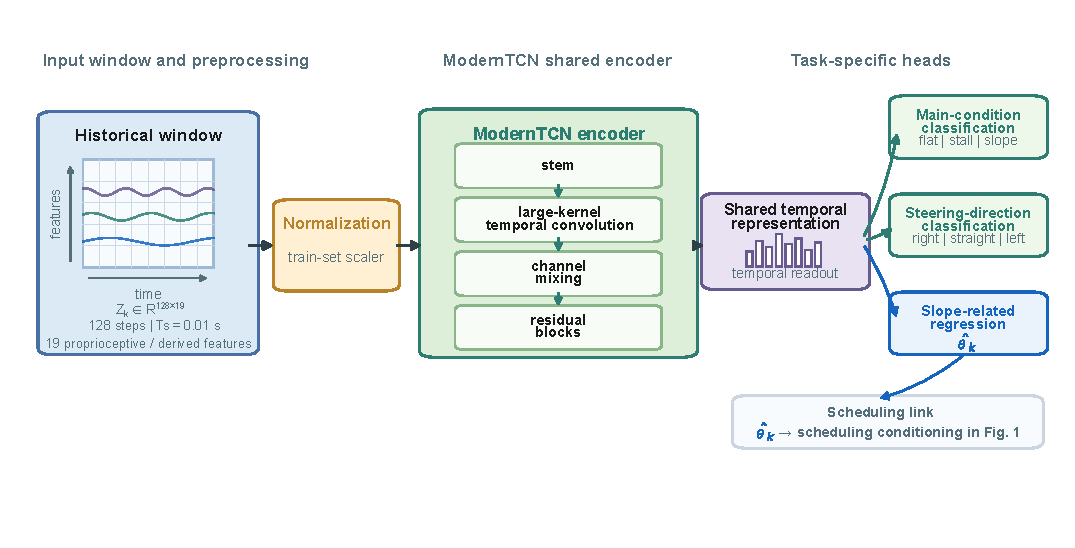
\includegraphics[width=\columnwidth]{fig04_temporal_estimator.pdf}
\caption{ModernTCN-based multi-task temporal estimator for LPV-MPC scheduling perception. A train-set-normalized historical window is encoded by the ModernTCN encoder and mapped to three task-specific heads for main-condition classification, steering-direction classification, and slope-related regression.}
\label{fig:temporal_estimator}
\end{figure}
\FloatBarrier

% ===== Table 3 placeholder =====
\begin{table}[H]
\centering
\fbox{\parbox{0.85\linewidth}{\centering Placeholder: Temporal perception input and task definition.}}
\caption{Temporal perception input and task definition.}
\label{tab:temporal_input}
\end{table}
\FloatBarrier



\subsection{ModernTCN-Based Multi-Task Estimator}



The proposed temporal estimator is a lightweight ModernTCN-based multi-task network. Its input is the normalized historical window $Z_k$, and its outputs are the main-condition probability, steering-direction probability, and slope-related regression value:

\begin{equation}
\hat{\mathbf{o}}_k
=
g_{\phi}(Z_k),
\quad
\hat{\mathbf{o}}_k
=
\left[
\hat{p}^{main}_k,\,
\hat{p}^{turn}_k,\,
\hat{\theta}_k
\right].
\label{eq:multi_task_estimator}
\end{equation}

where $g_{\phi}(\cdot)$ denotes the trained temporal estimator. As shown in Fig.~\ref{fig:temporal_estimator}, the normalized input window is processed by a ModernTCN encoder and then mapped to three task-specific heads.

The network follows the general design idea of modern temporal convolutional models \citep{}. Large-kernel temporal convolution is used to extract history-dependent patterns, while pointwise channel mixing is used to capture coupling among different vehicle signals. A generic residual temporal block can be written as

\begin{equation}
H^{(\ell+1)}
=
H^{(\ell)}
+
\mathcal{M}^{(\ell)}
\left(
\mathcal{T}^{(\ell)}
\left(H^{(\ell)}\right)
\right),
\label{eq:temporal_block}
\end{equation}

where $\mathcal{T}^{(\ell)}(\cdot)$ denotes temporal convolution, and $\mathcal{M}^{(\ell)}(\cdot)$ denotes channel mixing and nonlinear transformation. The residual connection helps stabilize the stacked temporal representation.



The shared temporal representation is then passed to three task heads. The classification heads output the main-condition and steering-direction probabilities, while the regression head outputs the slope-related scheduling estimate. The network is not used as a direct controller. Its output is used only to assist LPV-MPC scheduling.



\subsection{Multi-Task Loss Function}



The temporal estimator is trained with a weighted multi-task loss,

\begin{equation}
\mathcal{L}
=
\lambda_{main}\mathcal{L}_{main}
+
\lambda_{turn}\mathcal{L}_{turn}
+
\lambda_{\theta}\mathcal{L}_{\theta},
\label{eq:multi_task_loss}
\end{equation}

where $\mathcal{L}_{main}$ and $\mathcal{L}_{turn}$ are classification losses for the main operating condition and steering direction, respectively, and $\mathcal{L}_{\theta}$ is the slope-regression loss. The weights $\lambda_{main}$, $\lambda_{turn}$, and $\lambda_{\theta}$ balance the three tasks.



This multi-task structure is adopted because the three outputs are related to the same underlying operating condition. Joint learning can encourage the shared temporal encoder to extract features that are useful for both condition recognition and slope scheduling estimation.



\subsection{Scheduling Conditioning}



The raw slope estimate is not directly used as a control input. Before entering the LPV-MPC scheduler, it is processed by a conditioning function:

\begin{equation}
\theta^{sch}_k = \mathcal{S}(\hat{\theta}_k),
\label{eq:scheduling_conditioning}
\end{equation}

where $\mathcal{S}(\cdot)$ includes magnitude limiting, rate limiting, and dead-zone filtering. The magnitude limit prevents unrealistically large scheduled slope values. The rate limit reduces abrupt changes in the scheduled model. The dead-zone prevents small slope fluctuations from unnecessarily changing the LPV model.



These safeguards are engineering measures to reduce scheduling discontinuities. They should not be interpreted as a formal stability proof. The constrained LPV-MPC remains the final controller that determines the AGV control command.



\subsection{Baseline Temporal Models}



Two temporal neural network baselines are considered. The first is GRU, which represents a recurrent sequence modeling method with gated memory. The second is conventional TCN, which represents a standard convolutional sequence baseline. Both baselines use the same input window, task definitions, and closed-loop controller as the proposed ModernTCN-based estimator. Therefore, the comparison focuses on whether the ModernTCN-based temporal representation provides better scheduling perception and closed-loop behavior under the same LPV-MPC framework. The main model configurations are listed in Table~\ref{tab:model_configs}.

% ===== Table 4 placeholder =====
\begin{table}[H]
\centering
\fbox{\parbox{0.85\linewidth}{\centering Placeholder: Model configurations of GRU, TCN and ModernTCN.}}
\caption{Model configurations of GRU, TCN and ModernTCN.}
\label{tab:model_configs}
\end{table}
\FloatBarrier



\section{Simulation-Based Closed-Loop Experimental Design}

\label{sec:experiment_design}



\subsection{Simulation Platform}



All closed-loop experiments are conducted on a MATLAB/Simulink simulation platform consisting of a nonlinear diagonal dual-steer AGV plant and an LPV-MPC controller. The nonlinear plant is used as the closed-loop simulation object, while the LPV-MPC controller uses the scheduled local prediction model for online optimization. The learning-based perception modules are called inside the closed-loop simulation to provide scheduling-related estimates.



The current study is simulation-based. No hardware-in-the-loop or physical AGV experiment is included. Therefore, the experimental conclusions should be interpreted as closed-loop simulation evidence rather than hardware deployment validation.



\subsection{Baseline Controllers and Estimators}



The compared controllers and estimators are summarized in Table~\ref{tab:baseline_definitions}. The zero-slope LPV-MPC baseline evaluates the performance of nominal scheduling. The IMU-based LPV-MPC baseline evaluates whether a simplified physical slope estimate is sufficient. The oracle LPV-MPC uses the true slope and provides an upper-bound reference for scheduling quality. GRU and TCN are learning-based temporal baselines. ModernTCN is the proposed temporal scheduling perception method. The causal ModernTCN is used only for ablation analysis.



\begin{table}[t]

\centering

\caption{Baseline controllers and estimators.}

\label{tab:baseline_definitions}

\begin{tabular}{lll}

\hline

Category & Method & Role \\

\hline

No-slope baseline & LPV-MPC theta0 & Nominal zero-slope scheduling \\

Sensor baseline & LPV-MPC IMU theta & Simplified sensor-based scheduling \\

Oracle baseline & LPV-MPC oracle theta & True-slope scheduling upper bound \\

Learning baseline & GRU & Recurrent temporal estimator \\

Learning baseline & TCN & Conventional convolutional estimator \\

Proposed method & ModernTCN & Multi-task temporal scheduling estimator \\

Ablation & Causal ModernTCN & Offline--closed-loop mismatch analysis \\

\hline

\end{tabular}

\end{table}

\FloatBarrier

\subsection{Closed-Loop Scenarios}



The closed-loop evaluation includes three route types, as shown in Fig.~\ref{fig:closed_loop_routes}. The first route is a factory logistics showcase path, which contains representative curved and sloped segments. The second route is a long up/down slope path, which emphasizes slope scheduling. The third route is a sharp turn transition path, which emphasizes the coupling between turning transition and slope-related scheduling.

% ===== Fig. 5 =====
\begin{figure*}[!t]
\centering

\includegraphics[width=\textwidth]{fig05_simulation_routes.pdf}
\caption{Closed-loop simulation routes used for evaluation: (a) factory logistics showcase, (b) long up/down slope, and (c) sharp turn transition. The arrows indicate the travel direction along the reference path.}
\label{fig:closed_loop_routes}
\end{figure*}
\FloatBarrier

These routes are used to test whether the proposed scheduling perception method is effective beyond a single trajectory. The factory logistics path is used as the main showcase route, while the other two routes are used for multi-route generalization and disturbance robustness evaluation.



\subsection{Disturbance and Robustness Settings}



Robustness is evaluated under designed disturbance levels. The nominal level corresponds to the baseline closed-loop simulation without additional disturbance. Higher disturbance levels introduce measurement noise and plant parameter perturbations. The perturbations include changes in vehicle and environment parameters that affect the closed-loop plant behavior.



The robustness study is intended to compare the relative closed-loop behavior of ModernTCN, GRU, and TCN under the same disturbance protocol. It does not cover all possible real-world sensor noise or plant uncertainty distributions. Broader validation with additional random seeds, real sensor noise, and hardware experiments remains future work.



\subsection{Evaluation Metrics}



The evaluation metrics are divided into four groups. The first group measures tracking performance:

\begin{equation}
\mathcal{M}_{track}
=
\left\{
e_{y,\mathrm{RMSE}},
e_{\psi,\mathrm{RMSE}},
e_{XY,\mathrm{RMSE}},
e_{y,\mathrm{peak}}
\right\}.
\label{eq:tracking_metrics}
\end{equation}

The second group measures control effort and smoothness:

\begin{equation}
\mathcal{M}_{control}
=
\left\{
J_{\Delta u},
F_{\mathrm{peak}},
\omega_{cmd,\mathrm{peak}}
\right\}.
\label{eq:control_metrics}
\end{equation}

The third group measures constraint behavior, including violation rate and saturation-related events. The fourth group measures perception and scheduling performance, including main-condition accuracy, steering-direction accuracy, slope-related error, and scheduled-slope smoothness.



Separating these metrics is important because some methods, such as zero-slope LPV-MPC and oracle LPV-MPC, are not classifiers. Therefore, perception metrics should be interpreted only for learning-based methods, while the oracle method should be interpreted primarily as a tracking and control upper-bound reference.



\subsection{Fairness and Reproducibility Protocol}



All learning-based methods use the same input features, same task definitions, same training and testing protocol, and same LPV-MPC controller. The temporal input length is $128$ steps, the input dimension is $19$, and the sampling time is $0.01~\mathrm{s}$. A run-level split is adopted to avoid placing highly overlapping windows from the same simulation run into both training and testing sets. The normalization statistics are fitted on the training set only and then applied to validation, test, and closed-loop inference.



This protocol is included to ensure fair comparison among GRU, TCN, and ModernTCN. It is not presented as a separate dataset contribution.



\subsection{Computational Feasibility Check}



A computational feasibility check is included to measure the core inference time of the temporal estimator and the MPC solve time. This experiment is used only as an implementation feasibility indicator. Since no embedded controller or physical AGV is tested, the timing result should not be interpreted as a hardware deployment validation. Desktop MATLAB/Simulink wrapper overhead is reported separately when applicable.



\section{Results and Discussion}

\label{sec:results_discussion}



\subsection{Does Scheduling Mismatch Matter?}



The main closed-loop comparison is designed to examine whether slope-related scheduling mismatch significantly affects LPV-MPC path tracking. Fig.~\ref{fig:main_route_comparison} shows the trajectory and tracking error comparison, and Table~\ref{tab:main_closed_loop} summarizes the main-route results for the proposed method and the baseline controllers. For readability, the XY trajectory panel includes all compared methods, whereas the lateral-error and heading-error panels focus on the learning-based methods and the oracle baseline. The large tracking errors of the zero-slope and IMU-based baselines are quantified in Table~\ref{tab:main_closed_loop}.

% ===== Fig. 6 =====
\begin{figure*}[!t]
\centering

\includegraphics[width=\textwidth]{fig06_main_closed_loop.pdf}
\caption{Main-route closed-loop comparison on the factory logistics showcase path: (a) XY trajectory of all compared methods, (b) lateral error of the learning-based methods and oracle baseline, and (c) heading error of the learning-based methods and oracle baseline. The zero-slope and IMU-based LPV-MPC baselines produce much larger tracking errors, which are quantified in Table~\ref{tab:main_closed_loop}.}
\label{fig:main_route_comparison}
\end{figure*}
\FloatBarrier



\begin{table}[t]

\centering

\caption{Main closed-loop results on the factory logistics showcase path.}

\label{tab:main_closed_loop}

\begin{tabular}{lrrrrrr}

\hline

Controller & $e_y$ RMSE & $e_{\psi}$ RMSE & XY RMSE & $J_{\Delta u}$ & Violation rate & $\theta^{sch}$ MAE \\

\hline

ModernTCN & 0.0246 & 0.0438 & 0.8036 & 0.5991 & 0 & 0.9239 \\

GRU & 0.0623 & 0.1714 & 1.6641 & 7.0298 & 0 & 0.3415 \\

TCN & 0.0364 & 0.1061 & 1.3538 & 235.6737 & $5.277\times 10^{-5}$ & 1.7077 \\

LPV-MPC theta0 & 26.2527 & 1.6517 & 32.0981 & 285.9290 & 0.1040 & 3.1339 \\

LPV-MPC IMU theta & 26.4718 & 1.6155 & 32.1210 & 285.8180 & 0.1040 & 2.9522 \\

LPV-MPC oracle theta & 0.0236 & 0.0315 & 0.5602 & 0.0609 & 0 & 0.0722 \\

\hline

\end{tabular}

\end{table}



The zero-slope and simplified IMU-based LPV-MPC baselines show large tracking errors on the showcase route. This indicates that the scheduled slope is not a negligible auxiliary signal on this route. When the LPV-MPC uses an inaccurate slope-related scheduling variable, the prediction model becomes inconsistent with the nonlinear plant and the resulting closed-loop path tracking deteriorates significantly.



The oracle LPV-MPC achieves the best scheduling reference because it uses the true slope. ModernTCN obtains a lateral-error RMSE close to the oracle result on the main path. This result suggests that the learned temporal perception module can provide useful scheduling information for LPV-MPC. However, the gap between ModernTCN and oracle remains visible in global position error and control smoothness. Therefore, the proposed method should be interpreted as an effective scheduling enhancement rather than a replacement for perfect slope information.



\subsection{Learning-Based Controller Comparison}



Among the learning-based controllers, ModernTCN provides the best overall closed-loop tradeoff on the main route. It achieves the smallest lateral-error RMSE, heading-error RMSE, and global position RMSE among GRU, TCN, and ModernTCN. It also maintains a low control smoothness cost and zero violation rate in the reported summary.



The comparison also shows that a single perception metric is not sufficient to rank the learning-based controllers. GRU obtains a smaller scheduled-slope MAE than ModernTCN on the main route, but its tracking errors are larger. TCN obtains favorable values in some local scheduling or steering-related metrics, but it shows a much larger control smoothness cost and a nonzero violation rate. Therefore, the conclusion is not that ModernTCN is uniformly superior in every single metric. Rather, ModernTCN gives the most robust overall closed-loop performance among the learning-based methods.



\subsection{Multi-Route Generalization}



Table~\ref{tab:multipath_aggregate} summarizes the aggregate results over three closed-loop routes. The benchmark includes the factory logistics showcase path, the long up/down slope path, and the sharp turn transition path.



\begin{table}[t]

\centering

\caption{Aggregate closed-loop results over three routes.}

\label{tab:multipath_aggregate}

\begin{tabular}{lrrrrrr}

\hline

Controller & Paths & $e_y$ RMSE mean & $e_{\psi}$ RMSE mean & XY RMSE mean & $J_{\Delta u}$ mean & Overall rank mean \\

\hline

ModernTCN & 3 & 0.0319 & 0.0321 & 0.4889 & 13.3133 & 1.0000 \\

LPV-MPC oracle theta & 3 & 0.0347 & 0.0294 & 0.3951 & 0.4386 & 2.0000 \\

GRU & 3 & 0.0483 & 0.0851 & 0.9358 & 3.3528 & 3.3333 \\

TCN & 3 & 0.0489 & 0.0814 & 1.0695 & 313.9197 & 3.6667 \\

LPV-MPC IMU theta & 3 & 8.8930 & 0.6669 & 12.1776 & 579.7648 & 5.0000 \\

LPV-MPC theta0 & 3 & 8.8276 & 0.6891 & 12.2527 & 644.0558 & 6.0000 \\

\hline

\end{tabular}

\end{table}

ModernTCN obtains the best mean overall rank across the three paths. This result reduces the possibility that the main-route result is caused only by trajectory-specific tuning. The oracle method remains a strong upper-bound reference in terms of global position error and control smoothness, but ModernTCN is the most consistent learning-based controller over the multi-route benchmark.



The multi-route results also show that the zero-slope and IMU-based LPV-MPC baselines remain weak on routes where slope scheduling is important. This supports the central motivation of the paper: reliable scheduling information is necessary for LPV-MPC path tracking under sloped and transitional conditions.



\subsection{Scheduling Behavior Analysis}

% ===== Fig. 7 =====
\begin{figure*}[!t]
\centering

\includegraphics[width=\textwidth]{fig07_scheduled_slope.pdf}
\caption{Scheduled-slope behavior on the factory logistics showcase path: (a) scheduled slope signals actually used by the LPV-MPC controller after conditioning and (b) scheduling error with respect to the true slope. The oracle baseline uses the true slope directly, while the zero-slope baseline keeps the scheduled slope at zero.}
\label{fig:scheduled_slope}
\end{figure*}
\FloatBarrier

Fig.~\ref{fig:scheduled_slope} compares the scheduled-slope signals actually used by the LPV-MPC controller. The oracle baseline follows the true slope, while the zero-slope and IMU-based schedulers show large scheduling errors over the sloped segments. Among the learning-based methods, ModernTCN does not always produce the smallest pointwise scheduled-slope error. In fact, GRU obtains a smaller scheduled-slope MAE on the main route, as reported in Table~\ref{tab:main_closed_loop}. However, its closed-loop tracking errors and control smoothness cost are larger than those of ModernTCN. This indicates that the closed-loop effect of a scheduling signal depends not only on pointwise slope accuracy, but also on its temporal behavior and interaction with the LPV-MPC prediction model and constraints.

Therefore, ModernTCN should be interpreted as providing the most favorable closed-loop scheduling behavior among the learning-based methods, rather than as the most accurate slope estimator at every instant. This observation is consistent with the broader conclusion that learning-enhanced MPC modules must be evaluated in closed loop rather than only by offline or pointwise perception metrics.



\subsection{Control Smoothness and Constraint Behavior}



Control smoothness and constraint behavior are important for evaluating a path-tracking controller. A controller that achieves low tracking error with excessive input variation may not be desirable for industrial AGV operation. Fig.~\ref{fig:control_smoothness} compares the command histories, normalized input increment, and constraint-related summary indicators on the factory logistics showcase path. The normalized input increment is computed as
\begin{equation}
\left\|\Delta u_k^{\mathrm{norm}}\right\|_2 =
\left\|
\left[
\frac{\Delta F_{\mathrm{cmd},k}}{\Delta F_{\max}},
\frac{\Delta \omega_{\mathrm{cmd},k}}{\Delta \omega_{\max}}
\right]
\right\|_2 ,
\end{equation}
where $\Delta F_{\max}=400~\mathrm{N}$ and $\Delta \omega_{\max}=0.9~\mathrm{rad/s}$ are the input-rate limits used for normalization. The max limit-hit ratio denotes the larger channel-wise percentage of samples that reach the active limit between the driving-force and yaw-rate command channels, while the violation rate denotes the percentage of samples outside the active input limits.

% ===== Fig. 8 =====
\begin{figure*}[!t]
\centering
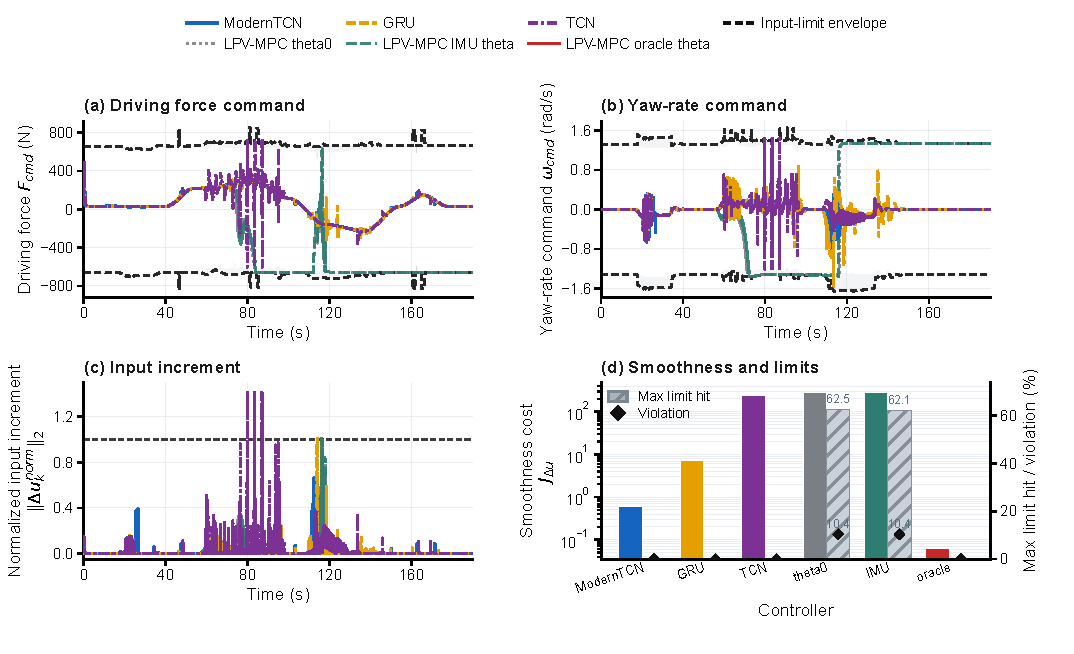
\includegraphics[width=\textwidth]{fig08_control_smoothness.pdf}
\caption{Control smoothness and constraint behavior on the factory logistics showcase path: (a) driving-force command, (b) yaw-rate command, (c) normalized input-increment metric, and (d) summary of smoothness cost $J_{\Delta u}$, max limit-hit ratio, and violation rate. The dashed black envelopes indicate the active command limits in (a) and (b), and the normalized input-increment limit in (c). In (d), the colored bars denote $J_{\Delta u}$, the hatched bars denote the max limit-hit ratio, and the black diamond markers denote the violation rate.}
\label{fig:control_smoothness}
\end{figure*}
\FloatBarrier

The results show that TCN can achieve competitive values in some perception metrics, but it produces a much larger input variation and control smoothness cost on the main route and in the multi-route aggregate. This indicates that local perception accuracy does not automatically translate into smooth closed-loop control. The zero-slope and IMU-based baselines frequently contact the active input limits and exhibit nonzero violation rates. The oracle LPV-MPC has the smallest control smoothness cost among the main-route methods because it uses the true slope for scheduling. ModernTCN is less smooth than the oracle, which suggests that residual slope-estimation error and scheduling discontinuity still affect the control input. Nevertheless, compared with the zero-slope and IMU-based baselines, ModernTCN substantially reduces both tracking error and constraint violations. This confirms that temporal scheduling perception improves not only the trajectory error but also the closed-loop control behavior.



\subsection{Robustness Under Disturbance and Parameter Perturbation}



Robustness is evaluated on two route types under three disturbance levels. Table~\ref{tab:robustness_aggregate} reports the aggregate results, and Fig.~\ref{fig:robustness_trend} visualizes the robustness trends. Each disturbance level contains the long up/down slope path and the sharp turn transition path.

\begin{table}[t]

\centering

\caption{Robustness aggregate results under disturbance levels.}

\label{tab:robustness_aggregate}

\begin{tabular}{llrrrrr}

\hline

Level & Controller & Cases & $e_y$ RMSE mean & XY RMSE mean & $J_{\Delta u}$ mean & Overall rank mean \\

\hline

0 & ModernTCN & 2 & 0.0355 & 0.3316 & 19.6704 & 1.0000 \\

0 & GRU & 2 & 0.0413 & 0.5716 & 1.5143 & 2.0000 \\

0 & TCN & 2 & 0.0552 & 0.9273 & 353.0426 & 3.0000 \\

1 & ModernTCN & 2 & 0.0618 & 1.2880 & 205.7775 & 1.0000 \\

1 & GRU & 2 & 0.0765 & 1.3874 & 307.3123 & 2.5000 \\

1 & TCN & 2 & 0.0686 & 1.4244 & 669.0800 & 2.5000 \\

2 & ModernTCN & 2 & 0.0819 & 1.6587 & 709.7600 & 1.0000 \\

2 & GRU & 2 & 0.1170 & 1.8842 & 292.1800 & 2.0000 \\

2 & TCN & 2 & 0.0957 & 1.8597 & 1101.8100 & 3.0000 \\

\hline

\end{tabular}

\end{table}

% ===== Fig. 9 =====
\begin{figure*}[!t]
\centering
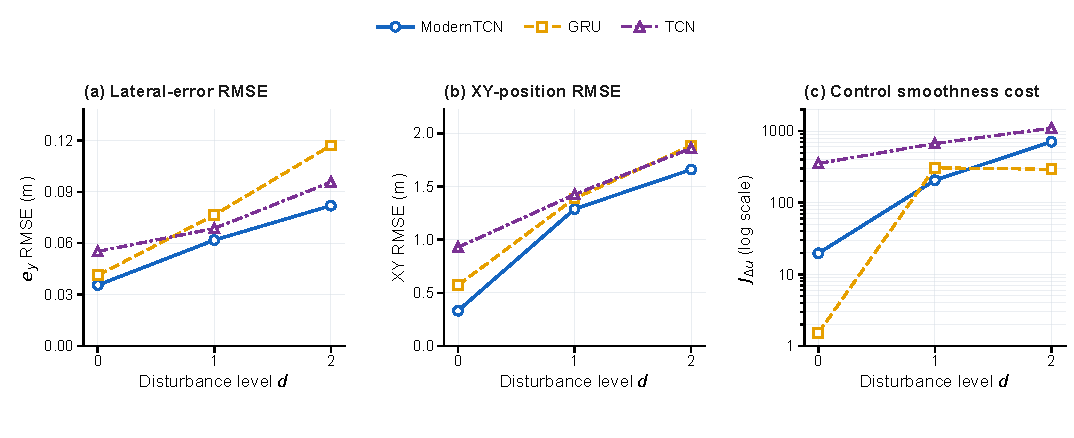
\includegraphics[width=\textwidth]{fig09_robustness.pdf}
\caption{Robustness trends of the learning-based controllers under disturbance levels $d=0,1,2$: (a) lateral-error RMSE, (b) XY-position RMSE, and (c) control smoothness cost $J_{\Delta u}$ on a logarithmic scale. The values are averaged over the long up/down slope and sharp turn transition routes.}
\label{fig:robustness_trend}
\end{figure*}
\FloatBarrier

As the disturbance level increases, the tracking errors generally become larger for the learning-based controllers. The control smoothness cost also increases clearly for ModernTCN and TCN, while GRU shows a non-monotonic variation in $J_{\Delta u}$. Although ModernTCN does not always yield the lowest smoothness cost, especially under the nominal condition, it consistently achieves the lowest tracking errors and the best overall rank across the tested disturbance levels. This result supports the relative robustness of ModernTCN under the designed disturbance settings.



The robustness result should be interpreted carefully. The disturbance cases are finite simulation scenarios, not a complete representation of all real-world uncertainties. Additional random seeds, real sensor noise, hardware-in-the-loop tests, and physical AGV experiments are needed for stronger robustness claims.



\subsection{Offline Perception Metrics Are Not Enough}



Offline perception metrics are useful for understanding the temporal estimator, but they are not sufficient for evaluating a learning-enhanced controller. In the offline test, the default ModernTCN achieves high main-condition and steering-direction accuracy. GRU achieves a competitive slope-related error in some metrics, while TCN can be locally competitive in steering-related metrics. However, their closed-loop results differ substantially.



This discrepancy occurs because closed-loop control introduces feedback. A local perception error can change the scheduled model, which changes the control action, which further changes the future vehicle state and input window. Therefore, the distribution encountered by the temporal estimator during closed-loop operation may differ from the offline test distribution. For this reason, offline classification accuracy and regression error should be treated as explanatory metrics rather than the primary evidence of control performance.



\subsection{Causal ModernTCN Ablation}



The causal ModernTCN ablation is included to examine whether a causal temporal padding design improves closed-loop robustness. Its offline metrics are close to the default ModernTCN in several aspects, as shown in Table~\ref{tab:causal_offline}. However, Fig.~\ref{fig:causal_mismatch} shows that its closed-loop tracking and smoothness metrics deteriorate substantially on the main route. This result indicates that the tested causal modification changes the feedback behavior of the scheduler, even though the window-level perception metrics remain competitive.

% ===== Table 9 placeholder =====
\begin{table}[H]
\centering
\fbox{\parbox{0.85\linewidth}{\centering Placeholder: Offline perception and causal ablation results.}}
\caption{Offline perception and causal ablation results.}
\label{tab:causal_offline}
\end{table}
\FloatBarrier

% ===== Fig. 10 =====
\begin{figure*}[!t]
\centering
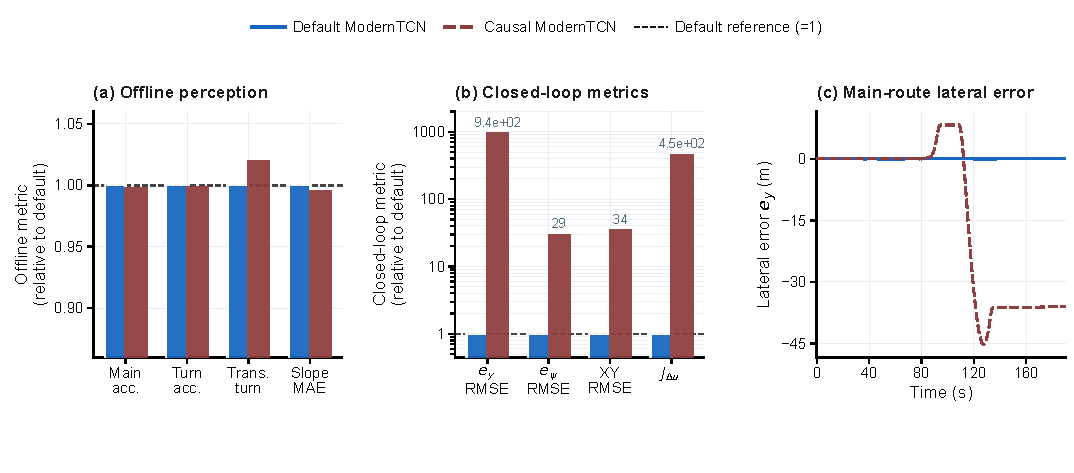
\includegraphics[width=\textwidth]{fig10_offline_closed_loop_mismatch.pdf}
\caption{Offline--closed-loop mismatch of the causal ModernTCN ablation: (a) offline perception metrics normalized by the default ModernTCN, (b) closed-loop metrics normalized by the default ModernTCN on a logarithmic scale, and (c) main-route lateral error. The dashed horizontal line in (a) and (b) denotes the default reference ratio of one. For offline metrics, larger values are better for the accuracy metrics, whereas smaller values are better for slope MAE.}
\label{fig:causal_mismatch}
\end{figure*}
\FloatBarrier

The causal variant remains close to the default model in offline perception metrics, but its closed-loop lateral tracking, global tracking, and control smoothness metrics degrade by one to three orders of magnitude. This result should not be interpreted as a general conclusion that causal temporal convolution is unsuitable for control. It only indicates that the particular causalization and training setting tested in this work did not produce robust closed-loop scheduling behavior. The more important conclusion is methodological: learning-enhanced MPC modules must be evaluated in the closed loop. For scheduling perception, temporal continuity, feedback-induced distribution shift, and control sensitivity are as important as window-level accuracy.



\subsection{Computational Cost}



A computational feasibility check is reported in Table~\ref{tab:realtime} to quantify the core inference and MPC solving cost. The result indicates that the core inference and MPC solve times are small compared with the control sampling period used in the simulation. However, MATLAB/Simulink desktop wrapper overhead is implementation-specific and should not be interpreted as embedded real-time performance.

% ===== Table 10 placeholder =====
\begin{table}[H]
\centering
\fbox{\parbox{0.85\linewidth}{\centering Placeholder: Computational feasibility check.}}
\caption{Computational feasibility check.}
\label{tab:realtime}
\end{table}
\FloatBarrier

Because no embedded controller, hardware-in-the-loop platform, or physical AGV experiment is included, the timing analysis is reported only as a computational feasibility indicator. A complete real-time deployment validation remains future work.



\subsection{Limitations}



Several limitations should be acknowledged. First, all results are based on MATLAB/Simulink closed-loop simulation. No hardware-in-the-loop or physical AGV experiment is included. Second, the current IMU-based scheduler is a simplified baseline and does not represent all possible sensor-fusion methods for slope estimation. Third, the disturbance study covers designed simulation perturbations, but it does not fully represent real sensor noise, actuator delay, floor irregularities, or hardware uncertainty.



Fourth, this paper does not provide a formal closed-loop stability proof for the learning-enhanced LPV-MPC system. The neural network output is conditioned before entering the LPV-MPC scheduler, and the MPC still handles input and input-rate constraints, but these mechanisms should not be interpreted as a rigorous stability guarantee. Finally, the current temporal estimator is trained and evaluated under the available simulation data distribution. Its generalization to real AGV measurements requires additional validation.



\section{Conclusion}

\label{sec:conclusion}



This paper proposed a multi-task temporal-perception-enhanced LPV-MPC framework for path tracking of a diagonal dual-steer AGV under sloped and turning-transition operating conditions, with abnormal resistance included as an auxiliary operating-condition perception target. The proposed method addresses the scheduling mismatch problem of LPV-MPC by estimating interpretable scheduling-related variables from historical proprioceptive measurements.



A lightweight ModernTCN-based estimator was adapted to jointly predict the main operating condition, steering direction, and slope-related scheduling variable. The estimated scheduling information was incorporated into the LPV-MPC update, while the final control action remained generated by the constrained model predictive controller.



Closed-loop simulation results showed that ModernTCN substantially improved tracking performance compared with zero-slope and simplified IMU-based LPV-MPC baselines. Compared with GRU and conventional TCN, ModernTCN provided the most robust overall closed-loop tradeoff across the main route, multiple routes, and designed disturbance levels. The oracle LPV-MPC results further indicated that ModernTCN approached the true-slope scheduling upper bound in lateral tracking, although gaps remained in global position error and control smoothness.



The causal ModernTCN ablation demonstrated that strong offline perception metrics do not necessarily lead to robust closed-loop control. This result highlights the necessity of closed-loop validation for learning-enhanced MPC systems. Future work will focus on hardware-in-the-loop and physical AGV experiments, real sensor noise validation, broader random-seed robustness tests, formal stability or error-bound analysis, and safer fallback strategies for uncertain scheduling conditions.


% Add the final IEEE bibliography here, or use:
% \bibliographystyle{IEEEtran}
% \bibliography{paper_v1_references}

\EOD
\end{document}
